\section{情報・金銭の流れ}
\subsection{情報の流れ}
本システムは,管理者端末,利用者端末の2つの端末と Amazon WebServise(AWS) 内の WEB/AP サーバ,データベースおよびストレージとそれを繋ぐインターネットによって構成されている.図 \ref{fig:Q7}に各端末とサーバが通信する情報の流れを示す.管理者,利用者は,必要な情報を AWS 内のデータベースなどに要求することで,情報の提供が行われ,要求に応じた各システムの処理が行われる.

\begin{figure}[H]
        \centering
        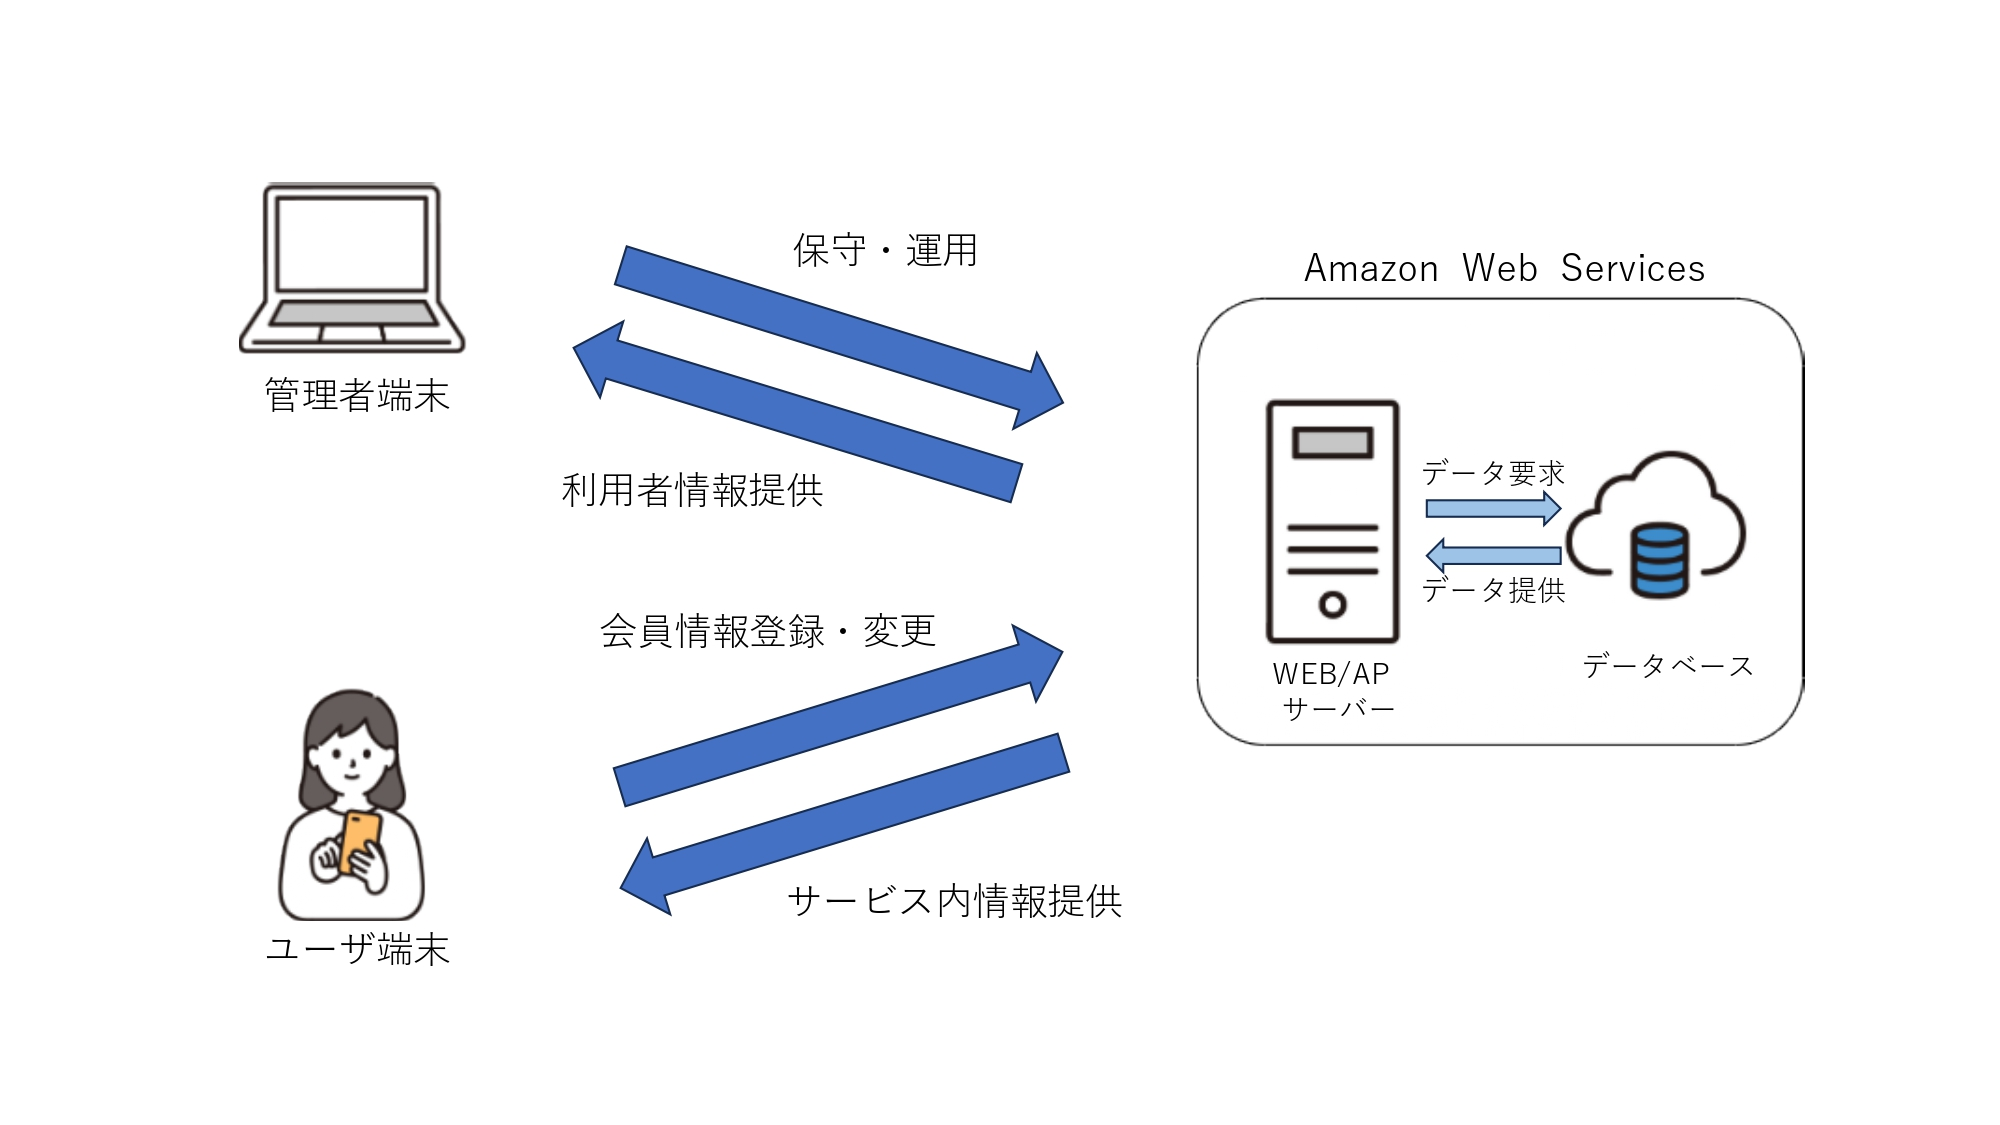
\includegraphics[width=12cm, height=7cm]{pictures/4-1_info.jpg}
        \caption{情報の流れ}
        \label{fig:Q7}
\end{figure}



\subsection{金銭の流れ}
金銭の流れは,図\ref{fig:Q8}に示す.

\begin{figure}[H]
        \centering
        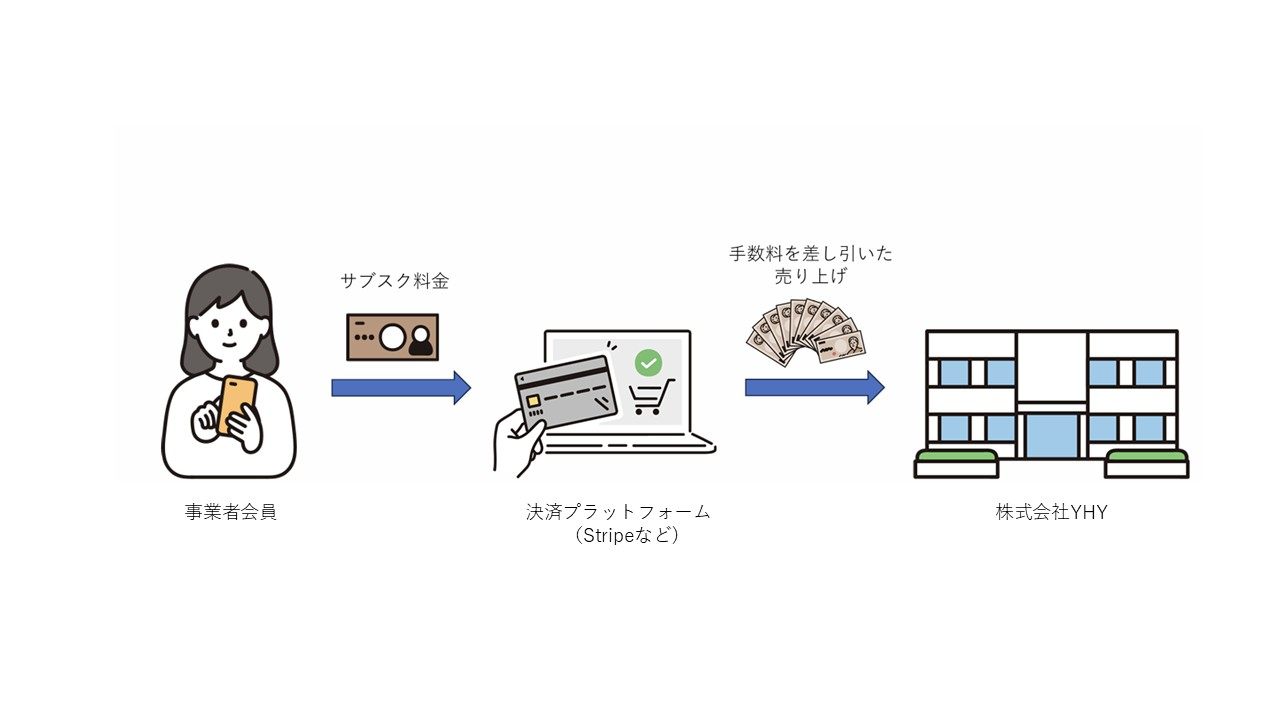
\includegraphics[width=12cm, height=7cm]{pictures/4-2_money.jpg}
        \caption{金銭の流れ}
        \label{fig:Q8}
\end{figure}

事業者会員は,クレジットカードなどを用いてサブスクリプション料金を支払う.この支払いは直接弊社に送金されるのではなく,決済プラットフォームを経由して処理される仕組みである。決済プラットフォームは,利用者から受け取った料金から決済手数料(数%程度)を差し引いたうえで、残額を弊社に振り込む.この入金は即時ではなく,一定期間(例:1 週間または 1 か月)分をまとめて支払われる.そのため,弊社が実際に受け取る金額は,利用者の支払総額から手数料を差し引いた純売上となる.







